\documentclass[serif,mathserif]{beamer}
\usepackage{amsmath, amsfonts, epsfig, xspace}
\usepackage{algorithm,algorithmic}
\usepackage{pstricks,pst-node}
\usepackage{multimedia}
\usepackage[normal,tight,center]{subfigure}
\setlength{\subfigcapskip}{-.5em}
\usepackage{beamerthemesplit}
\usetheme{lankton-keynote}

\author[Ingo Fischer]{Ingo Fischer}

\title[Messaging\hspace{2em}\insertframenumber/\inserttotalframenumber]{Messaging}

\date{} %leave out for today's date to be insterted

\institute{ProfitBricks GmbH}

\begin{document}

\maketitle

% \section{Introduction}  % add these to see outline in slides

\begin{frame}
\frametitle{Main Concepts}
Besides choosing a Message Protocol and the corresponding Messaging Architecture, 
we should define some main concepts that are independent of the Messaging solution we choose.
\end{frame}

\begin{frame}
\frametitle{Main Concepts}
\begin{itemize}
  \item Completely abstract underlying transport mechanism
  \begin{itemize}
    \item separate transport logic
    \item configure transport with configuration files
    \item Service lookup (how?)
    \item later: allow dynamic change of transport without
    restarting/reconfiguring services (how?)
  \end{itemize}
\end{itemize}
\end{frame}

\begin{frame}
\frametitle{Main Concepts}
Provide multiple communication channels, or stick with one?
\begin{itemize}
  \item Socket (backward compatiblity)
  \item AMQP/STOMP
  \item JMS
  \item SOAP, REST
  \item XMPP
\end{itemize}
\end{frame}

\begin{frame}
\frametitle{Messaging Protocols}
Messaging Protocols
\begin{itemize}
  \item AMQP
  \item STOMP
  \item 0MQ
  \item JMS
\end{itemize}
\end{frame}

\begin{frame}
\frametitle{Main questions}
We have to ask ourselves some important question in order to choose the messaging solution:
\begin{itemize}
  \item Do we need reliable messaging? (no \O MQ) 
  \item Do we need persistent messages? (no \O MQ)
  \item Do we need brokerless architecutes (\O MQ)
  \item Do we need performance (\O MQ)
  \item Do we need combinations of above? (OMG)
  \item Will we choose the better solution if it has a steeper learning curve?
\end{itemize}
\end{frame}

\begin{frame}
\frametitle{STOMP}
STOMP
\begin{itemize}
  \item 
\end{itemize}
\end{frame}

\begin{frame}
\frametitle{STOMP}
OpenWire
\begin{itemize}
  \item 
\end{itemize}
\end{frame}

\begin{frame}
\frametitle{AMQP}
AMQP
\begin{itemize}
  \item Open Standard Application Layer Protocol
  \item Describes message orientation, queuing, routing (point to point,
  pubsub), reliability and security
  \item Mandate behaviour of messaging provider and client
  \item Binary Wire level protocol
  \item Clients are mostly written against C API
  \item Mostly used by Banks
  \item Replace handbuild messaging/TCP connections
  \item Replace ALL kind of inter- and cross-application communication
\end{itemize}
\end{frame}

\begin{frame}
\frametitle{\O MQ}
\O MQ
\begin{itemize}
  \item ``Sockets on Steroids''
  \item ``\O MQ is AMQP done right''
  \item By Imatix
  \item Extends Socket API
  \item Concurrency, Queuing, High Availability
  \item No builtin Message reliability (like with AMQP)
  \item Extremely fast, used for distributed computations
  \item Faster than TCP (Supercomputing)
  \item Allows inprocess, IPC, TCP and Multicast messaging
  \item ``Put workers anywhere you like''
\end{itemize}
\end{frame}

% Pro ZeroMQ, Contra AMQP arguments: http://twit.tv/show/floss-weekly/195

% ZeroMQ users:
%   Mongrel2: http://mongrel2.org/, a language independent Web Server
%   Salt, Saltstack

\begin{frame}
\frametitle{Messaging Protocols}
\O MQ
\begin{itemize}
  \item Born because AMQP was handed over to industry
  \begin{itemize}
    \item development of AMQP really slow
    \item Creator of AMQP says ``I would never implement that'' %http://twit.tv/show/floss-weekly/195, 13:10
    \item AMQP is a dead protocol
  \end{itemize}
  \item Allows brokerless architectures (mostly multiple queues are built up)
  \item used in iPython 0.12+, Loggly (large scale distributed logging)
  \item not a daemon, not a Server, just a library
\end{itemize}
\end{frame}

\begin{frame}
\frametitle{\O MQ}
\O MQ
\begin{itemize}
  \item
  \item CAN be a message queue
  \item Created for Stock markets
  \item Almost no protocol overhead (just plain content + small header),
  Messages of all kinds can be send (imagine sending VM images!)
  \item Supports PGM, a reliable multicast transport protocol
  \item Idea: build as many hops as you need, because they're cheap and simple
  \item No builtin persistence
  \item Good to plug different languages together
  \item \O MQ only handles connection re-establishment, will not resend message if the message is lost
\end{itemize}
\end{frame}

\begin{frame}
\frametitle{\O MQ}
\O MQ - conclusion
\begin{itemize}
  \item
  \item Learning how to use a decentralized model can be very confusing, in contrast to a centralized, broker-based
  architecture based on AMQP
  \item Hard to understand
\end{itemize}
\end{frame}

\begin{frame}
\frametitle{Other Protocols}
Protocol Buffers
\begin{itemize}
  \item Protocol Buffers are a way of encoding structured data in an efficient yet extensible format.
  Google uses Protocol Buffers for almost all of its internal RPC protocols and file formats.
\end{itemize}
\end{frame}

\begin{frame}
\frametitle{Message Brokers}
Message Brokers
\begin{itemize}
  \item RabbitMQ
  \item ActiveMQ
  \item ActiveMQ Apollo (Beta, Rewrite of ActiveMQ)
\end{itemize}
Alternatives (or usage in combination with Messaging?)
\begin{itemize}
  \item Apache Zookeeper
  \item Puppet Libvirt Plugin
  \item Salt
\end{itemize}
\end{frame}

\begin{frame}
\frametitle{RabbitMQ}
RabbitMQ
\begin{itemize}
  \item Only 100\% AMQP Provider
  \item Based on Erlang/OTP
  \item owned by VMWare
  \item whitespread
  \item Supports STOMP protocol, but only through a Plugin (with some issues currently)
\end{itemize}
\end{frame}

\begin{frame}
\frametitle{ActiveMQ}
ActiveMQ 5.5
\begin{itemize}
  \item Written in Java
  \item JMS, STOMP, OpenWire (No AMQP) 
  \item Pro:
  \begin{itemize}
    \item Java application: internal administration knowhow available
    \item JAAS authentication
    \item Can be deployed to Glassfish
    \item Good testability: can be used in-memory inside unit/component tests
    \item Support for JMS, which we already use for E-Mail and Billing Events
	\item Easy Migration to successor, ActiveMQ Apollo
  \end{itemize}
\end{itemize}
\end{frame}

\begin{frame}
\frametitle{ActiveMQ}
ActiveMQ Apollo
\begin{itemize}
  \item Available as Beta 6
  \item Currently supports only STOMP Protocol
  \item Fastest STOMP Message Broker
  \item Build around modern non-blocking concepts
  \item Will receive JMS-support later
\end{itemize}
\end{frame}





% \section{Main Body} % add these to see outline in slides

% \begin{frame}
%   \frametitle{Equations}
%   Equations are easy
%   \begin{itemize}
%   \item Just and paste equations\pause
%   \item From the paper!
%     \begin{equation*}
%       \textbf{p}^* = \underset{\textbf{p}}{\arg\!\min}~\sum_{\textbf{x}}\left[ I(\textbf{W}(\textbf{x};\textbf{p})) - T(\textbf{x}) \right]^2
%     \end{equation*}
%   \end{itemize}
% \end{frame}

\begin{frame}
\frametitle{Zookeeper}
``A Distributed Coordination Service for Distributed Applications''
It exposes a simple set of primitives that distributed applications can build
upon to implement higher level services for synchronization, configuration maintenance,
and groups and naming. It is designed to be easy to program to, and uses a data model
styled after the familiar directory tree structure of file systems. It runs in Java and
has bindings for both Java and C.

\end{frame}

\begin{frame}
\frametitle{Zookeeper}
\begin{itemize}
  \item Created to configure large amount of Hadoop clusters
  \item Informations are replicated spread across multiple Servers
  \item Distributed processes coordinate through a shared hierarchical
  namespace, similar to a filesystem
  \item One Server is leader, leader is changed on failures
\end{itemize}

\end{frame}

\begin{frame}
\frametitle{Zookeeper}
\begin{figure}[t]
\centering
\subfigure[Overview]{
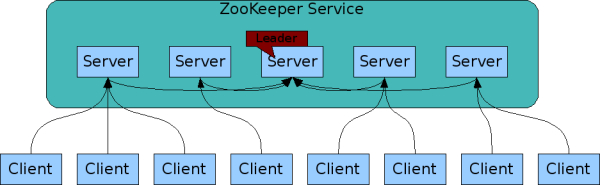
\includegraphics[width=10cm]{images/zkservice}}
%     \subfigure[Middle Frame]{
%     \includegraphics[width=3cm]{figures/naked_leaves/00000120}}
%     \subfigure[Last Frame]{
%     \includegraphics[width=3cm]{figures/naked_leaves/00000240}}
\end{figure}
\end{frame}

% \begin{frame}
%   \frametitle{A Movie}
%   \begin{center}
%     \movie[height=5cm,width=6.5cm,poster,autostart,loop]{}{leaves.avi}
%   \end{center}
%   \begin{itemize}
%   \item Movies only seem to work in Adobe Reader
%   \item Movie file is not embedded, it must be on the computer
%   \end{itemize}
% \end{frame}

% \section{Conclusion} % add these to see outline in slides

% \begin{frame}
%   \frametitle{Credits}
%   \begin{itemize}
%   \item Brought to you by www.shawnlankton.com
%   \item Please let me know about improvements!
%   \item This was supposed to look like a KeyNote Show
%   \item inspiration: http://www.ucl.ac.uk/~ucbpeal/latexposter.html
%   \item inspiration: http://newsgroups.derkeiler.com/... (in code)
%         %http://newsgroups.derkeiler.com/Archive/Comp/comp.text.tex/2007-11/msg00299.html
%   \end{itemize}
% \end{frame}

\begin{frame}
\frametitle{Questions}
\end{frame}
\end{document}